
%\newif\ifnote
%\ifx\notepaper\undefined
%  \notefalse
%\else
%  \notetrue
%\fi

\newcommand{\pflist}
  {	\renewcommand{\labelitemi}{$\triangleright$}
	\setlength{\itemsep}{0mm}
	\setlength{\parsep}{0mm}
	\setlength{\partopsep}{0mm}
	\setlength{\topsep}{0mm}
	\setlength{\parskip}{0mm}    }

\documentclass[a4paper]{article}

%\usepackage{afterpage}
\usepackage[dvips]{graphicx}
\usepackage{psfig}
\usepackage{fullpage}
%\usepackage{color}
\usepackage{pstricks}
%\usepackage{code}

\newcommand{\chapquotea}{notset}

\newenvironment{chapquote}[1]{\renewcommand{\chapquotea}{#1}\begin{quote}\it}{{\rm \hspace*{\fill}~\cite[]{\chapquotea} } \end{quote} \noindent}

\newenvironment{fragment}{\vspace{2mm}\begin{code}}{\end{code}\ \\}

%\newenvironment{fragment}{\begin{quote}\begin{code}}{\end{code}\end{quote}}

\newcommand{\citep}{\cite}

\newcommand{\dgrs}{$^{\circ}$}

\newcommand{\percent}{\%}

\newcommand{\ctt}[1]{``{\blue \tt #1}''}



%%\newcommand{\blue}{}

\begin{document}


\title{Dr. YARP\\ Doc{\small umentation} for Yet Another Robot Platform}


\author{Paul Fitzpatrick, Giorgio Metta}

\maketitle


\begin{center}
{\LARGE 

THIS ISN'T EVEN A DRAFT YET

\ \\

\ \\

don't believe a word you read here
}
\end{center}

\newpage


%YARP's communication code is, at heart, simply about moving bytes
%along pipes between processes, where the individual pipes and
%processes can be created and destroyed with minimal impact on the
%rest of the system.  For other communication models, YARP is not
%the tool to use -- try ACE/TAO for example.

\section{Getting started}

Make sure you have installed libYARP\_OS as described in Section~\ref{sect:install}.
We will now exercise your installation to make sure everything
is okay and correctly configured.  First, please open two terminal
windows; we'll refer to these as A and B.  

Before doing any communication, is is necessary to start the YARP name
service -- this is a program which keeps track of what YARP resources
are currently available and how to access them.
%
In terminal A, type:

\begin{verbatim}
yarp-service --run
\end{verbatim}

If all goes well, you will see a series of messages finishing in ``***
YARP name service started OK'' -- if not, check the configuration file
mentioned in the messages, or follow the advice given.

Next, in terminal B, type:
%
\begin{verbatim}
yarp-service --check
\end{verbatim}
%
This will try to communicate with the name server, send a message,
receive a message, and basically make sure that everything is
working well.  Here is what happens when all is well:

{\small
\begin{verbatim}
=================================================================
=== Trying to register some ports
*** making port /yarp-service/1 on default network [tcp, 11 ports]
*** making port /yarp-service/2 on default network [tcp, 11 ports]
=================================================================
=== Trying to connect some ports
*** connecting /yarp-service/1 to /yarp-service/2
=================================================================
=== Trying to write some data
*** Writing number 42
=================================================================
=== Trying to read some data
*** Read number 42
=================================================================
=== Trying to unregister some ports
=================================================================
*** YARP seems okay!
\end{verbatim}
}

If everything is okay, the last message wiil be ``*** YARP seems
okay!'' -- otherwise it will give some advice.  
Here is an example of things going wrong:

{\small
\begin{verbatim}
=================================================================
=== Trying to register some ports
*** making port /yarp-service/1 on default network [tcp, 11 ports]
*** FAILED port /yarp-service/1 - is the YARP name server running?
*** making port /yarp-service/2 on default network [tcp, 11 ports]
*** FAILED port /yarp-service/2 - is the YARP name server running?
=================================================================
=== Trying to connect some ports
==================================================================
=== Trying to write some data
*** Writing number 42
=================================================================
=== Trying to read some data
=== Trying to read some data
=== Trying to read some data
=================================================================
=== Trying to unregister some ports
=================================================================
*** YARP seems broken.
*** Check the configuration file at [/home/paulfitz/.yarp/conf/namer.conf]
*** It currently specifies a server at:
                Machine [wuffles]
                Port number [10000]
*** These settings can be changed on the first line of the file.
*** Perhaps try using an IP address instead of a host name.
***
*** If this is the wrong configuration file,
***    please set the optional YARP_ROOT environment variable
***    to the directory in which the desired namer.conf resides
***
\end{verbatim}
}

If networking is broken on your machine, then YARP will have trouble.
If you are running the YARP name server on a machine that does not
have a static IP address or a name registered with DNS, then you
should check the configuration file mentioned by yarp-service, and
make sure that the first line of the configuration file is of the form:
\begin{quote}
  current.valid.ip.address 10000
\end{quote}

The number ``10000'' is the default port number that the YARP name
service uses.  This is usually fine; if you have a conflict with this,
then please change it in the configuration file.

If all is well, we can try exercising YARP a little more.

In terminal B, type:
%
\begin{verbatim}
yarp-read /port1
\end{verbatim}
%
This will report \ctt{making port /port1 ...} in terminal B and in
terminal A some corresponding message will also appear.

Next, in terminal C, type:

\begin{verbatim}
yarp-write /port2
\end{verbatim}

If all goes well, this will report \ctt{making port /port2} in
terminal C and in terminal A some corresponding message will also
appear.

Now, in terminal D, type:

\begin{verbatim}
yarp-connect /port2 /port1
\end{verbatim}

Terminal C will report \ctt{connecting /port2 to /port1}.  Now if
you type ``hello world'' into terminal C, and hit enter, that text
will appear on terminal B.

If you have another computer with YARP installed on it, open a
terminal on it (let's call that terminal E) and type:

\begin{verbatim}
yarp_name_service machinename
\end{verbatim}

where machinename is the full name or IP address of the first machine
on which the YARP name service is running.  If all goes well it should
report \ctt{connection established with YARP name service running on
{\bf machinename}}.

Now on terminal E type:
%
\begin{verbatim}
yarp_read /port3
\end{verbatim}
%
and on terminal C, type:
%
\begin{verbatim}
yarp_connect /port2 /port3
\end{verbatim}
%
Now any line you enter in terminal B should appear in both terminal C and E.



\subsection{Getting coding}

Suppose you have a structure \ctt{Target} in process A with some data
you would like to have in process B:
%
\begin{verbatim}
struct Target {
  int x, y, z;
  char label[20];
};
\end{verbatim}
%
If you are operating in a homogeneous network (same OS and hardware on
all machines), then moving Target structures around is easy.  See
section XXX for a few details needed otherwise.
%
The steps are create, register, communicate, unregister (optional).
The necessary methods and classes are in the following header file:

\begin{verbatim}
#include <yarp/YARPPort.h>
\end{verbatim}
%
Make sure that YARP is set up okay on the machines you are using by 
running \ctt{yarp-service --check}.  If not, go to section XXX.
%
In process A you would create an output port that can send a Target:
%
\begin{verbatim}
YARPOutputPortOf<Target> out_port;
\end{verbatim}
%
%
In process B you would create an input port that can receive a Target:
%
\begin{verbatim}
YARPInputPortOf<Target> in_port;
\end{verbatim}
%
Then, in the main() methods of each process, you would create a name
for each port so that they can find each other.  For example, in
process A:
%
\begin{verbatim}
out_port.Register("/target/out");
\end{verbatim}
%
and in process B:
%
\begin{verbatim}
in_port.Register("/target/in");
\end{verbatim}
%
Once both processes are running, these ports can be connected by
typing \ctt{yarp-connect /target/out /target/in} on the command line.
Alternatively, you can connect them using code; for example, from
process A call:
%
\begin{verbatim}
out_port.Connect("/target/in");
\end{verbatim}
%
Now the ports are connected and ready to communicate.  In process A
you could set up a Target as follows:
%
\begin{verbatim}
Target& target = out_port.Content();
target.x = target.y = target.z = 10;
strncpy(target.label,"hello yarp world",sizeof(target.label));
\end{verbatim}
%
And then you could send it like this:
%
\begin{verbatim}
out_port.Write();
\end{verbatim}
%
In process B, you can wait for the Target to arrive by calling Read():
%
\begin{verbatim}
bool success = in_port.Read();
\end{verbatim}
%
If a target is successfully read, it becomes available using Content():
%
\begin{verbatim}
if (success) {
  Target@ target = in_port.Content();
  cout << "target is located at (" << target.x
       << "," << target.y
       << "," << target.z
       << ") with label " << target.label << endl;

}
\end{verbatim}

See Appendix XXX and demos in directory YYY for this code.


\subsection{The details}

Quality of service. 

Crossing OS/Hardware/Compiler boundaries.

Different protocols -- shared mem, tcp, udp, multicast.



\subsection{Messages in bottles}

When completely maximal efficiently is not a concern, it can be 
convenient to not have to compile the type of every message.
For this, the \ctt{YARPBottle} class is available.  This is a generic
container into which you can throw integers, floating point numbers,
and strings, send them across the network, then easy parse the message
again at the far side.  For example, the following code:
%
\begin{verbatim}
#include <stdio.h>

#include <yarp/YARPPort.h>
#include <yarp/YARPBottle.h>

int main() {
  YARPOutputPortOf<YARPBottle> out_port;
  out_port.Register("/test/demo00");
  out_port.Connect("/test/reader");

  for (int i=0; i<5; i++) {
    char buf[256];
    sprintf(buf,"test number %d", i);
    out_port.Content().writeText(buf);
    out_port.Write(1);
  }
  out_port.FinishSend();

  return 0;
}
\end{verbatim}
%
will send a series of YARPBottles out on the port \ctt{/test/demo00}.
If, before starting this code, you start a reader in another terminal with:
%
\begin{verbatim}
yarp-read /test/reader
\end{verbatim}
%
then the following messages should appear:
%
test number 0
test number 1
test number 2
test number 3
test number 4
%
The \ctt{yarp-read} reader responds to YARPBottles that contain text.
You can look at the source of yarp-read as an example of how to read 
a YARPBottle.

explain: Write(1), FinishSend



\newpage

\section{Installation}

\label{sect:install}

We suggest that, if you are a first-time user of YARP, you install it
on one or two machines first, before trying to set it up for a cluster.

To set YARP up on a single machine, first install the ACE library,
then libYARP\_OS, then test your installation before moving on to 
other YARP components.  To set YARP up on a cluster, you may 
wish to place ACE and the YARP libraries in a common shared directory
rather than installing on each machine.  We have a few tips for this 
process, particularly if you are using multiple operating systems (as
is common because of hardware support constraints).

\subsection{Why doesn't YARP follow installation standards?}
You might be wondering why we haven't set things up as in many existing open source packages. A short answer is that dealing with multiple operating systems is messy and we haven't found any neat and clean way of doing it. The best we came about is using perl for preparing the installation. See section \ref{sect:perl}.

\subsection{Perl scripts}
\label{sect:perl}

YARP uses perl scripts for configuration and installation. We chose to do so to make compilation on Windows and Unixes as uniform as possible in spite of the differnce between makefiles and Microsoft Developer Studio project files. Perl is generally available on Linux and available for Windows in a very nice free distribution. Check the following website:

\begin{quote}
{\tt http://www.activestate.com/Products/ActivePerl/}
\end{quote}

At the moment of writing we use version 5.8.4.810. Once intalled, please make sure the environment variables are properly registered so that you can run perl from the command line.
Type \ctt{perl} on the command line to check whether it works.

\subsection{Prerequisites to installation}

First of all, configure a CVS client as explained in SourceForge (http://www.sf.net).
You need to choose a directory (the prospective \$YARP\_ROOT) where to download the
YARP source code. Make sure you check the ``prune'' flag in CVS so you don't create
empty directories. In Windows you might want to use WinCVS.

I used WinCVS 1.3.something that solves the annoying timezone-daylight saving time
problem. I used also putty (and plink) as a ssh client for WinCVS. I found this
configuration very stable and I strongly suggest replicating it if you're not an expert. 
If you decide to use putty make sure you download all the small applications that come with the main terminal application. You will need a few of them during the configuration procedure (e.g. putty, pagent, and plink).

Make sure you do not change the default from the putty terminal application (ssh)
because it applies to plink too. Please, also configure and upload the public-private key as requested by SourceForge (unless you're an anonymous user). Make sure your CVS ssh connection is functional before moving to the next section. Since we're checking prerequisites here, download ACE 5.4.2 from:

\begin{quote}
{\tt http://www.cs.wustl.edu/~schmidt/ACE.html}
\end{quote}

It comes as a single {\em tar.gz} file that you can open both in Linux and Windows. Keep it handy since we're going to use it again. YARP includes now header files (from cvlibrary) and DLL for the Intel IPL (optionally used in image processing) in the repository so you no longer need to download and install them separately.

DLLs from Visual Studio 6.0: strangely enough the default install doesn't have the
correct version (e.g. the C terminal library wouldn't normally work. This applies to
NT4.0; I haven't investigated the issue on 2K or XP. If you're running NT4.0 you might
need to install Visual Studio on each machine of the network to get the DLLs right.

Please spend some time reading the SourceForge documentation on the use of CVS and
the WinCVS documentation. You should become acquainted with the different checkout
options and with the WinCVS configuration. It will definitely help later during
development.

Directories cannot be removed from the CVS server. Make sure you know what
you're doing when adding a new directory to the repository (admitting you're allowed to).
For Windows users, your machine should have the Visual Studio 6.0 installed and properly
service packed.

A few environment variables are required to properly compile YARP. The perl scripts will check whether \$YARP\_ROOT is defined and complain otherwise. Also, many applications rely on having a \$YARP\_ROOT defined to locate configuration files. You're requested to define:
\begin{itemize}
\item \$YARP\_ROOT (\%YARP\_ROOT\% in Windows) environment variable (e.g. \ctt{export YARP\_ROOT=/usr/src/yarp}).
\item and then add to path \$YARP\_ROOT/bin/(your OS)/ (location of binaries and DLLs), and of course substitute the forward slash with the backslash where appropriate.
\item add also to the path: \$YARP\_ROOT/scripts (and the subdirectories you need). In Windows I tend to prefer adding them to the �system� environment and not to the current user only.
\end{itemize}

On Windows you have to check you can run the developer studio from the command line. The usual check is \ctt{msdev}. If it fails then you might need to go and look at {\em VCVARS32.bat} and run it from your terminal. The {\em VCVARS32.bat} script prepares the environment to run visual studio and compile from the command line.

On Unixes (or Qnx) you can add the environment initialization in the {\em .profile}. An example of a plausible environment initialization is shown below. As you can see ACE on Unixes requires the definition of the \$ACE\_ROOT environment variable.

\begin{verbatim}
export YARP_ROOT=/usr/src/yarp
export ACE_ROOT=$YARP_ROOT/src/ACE_wrappers
export CVSROOT=:ext:youruser@cvs.sourceforge.net:/cvsroot/yarp0
export CVS_RSH=/usr/bin/ssh
export LD_LIBRARY_PTH=/usr/local/lib
export PATH=$PATH:$YARP_ROOT/bin/qnx6:$HOME/bin
export PATH=/usr/local/bin/:$PATH
export PATH=.:/lib:$PATH
\end{verbatim}

A brief checklist on this procedure is provided here for convenience:
\begin{enumerate}
	\item Download \& install the CVS client and configure your sourceforge user.
	\item Checkout YARP \ctt{cvs checkout yarp -P} somewhere on your directory tree (this will be your \$YARP\_ROOT.
	\item Install perl if your operating system requires to do so (e.g. Windows).
	\item Download ACE, possibly version 5.4.2. I tend to like the tar.gz file that has Unix-like newline characters.
	\item Setup environment variables as explained above.
\end{enumerate}

\subsection{Getting acquainted with the YARP directory tree}
The YARP directory tree contains the usual src, lib, bin, etc. subdivision. There are a few differences from a standard distribution since many libraries are created and several operating systems supported. A quick tour is the following table:

\begin{table}[h]
	\centering
		\begin{tabular}{|c|c|c|}
		\hline
			Directory name & Description \\
			\hline \hline
			bin & binaries with subdirectories for multiple OS \\
			\hline
			conf & configuration files, templates, etc. \\
			\hline
			docs & installation manuals, tutorial and other documents \\
			\hline
			include & header files are moved here after compilation of libraries \\
			\hline
			lib & libraries are moved here after compilation \\
			\hline
			packaging & scripts for creating the YARP distributions (does not concern the user) \\
			\hline
			scripts & scripts of various robotic experiments (not too neat to have them here) \\
			\hline
			src & the main source subdirectories including libraries, tools and experimental code \\
			\hline
		\end{tabular}
\end{table}


\subsection{Installing the ACE library}
\label{sect:ace}

We require ACE version 5.3.3 or greater (but we recommend 5.4.2 -- beta). There are two alternatives for compiling ACE: i) follow the ACE installation instructions, and ii) allow the YARP perl scripts to compile ACE for you -- the latter works only with ACE 5.4.2.

If you are taking the first route, on Debian-based linux machines, ACE is available as a binary package; simply type ``apt-get install libace-dev'' as super-user.  Please
check (e.g. by searching at {\tt http://packages.debian.org}) that the version available is 5.3.3 or greater.  At the time of writing, this is true for Debian unstable but not true for Debian stable.

For all other scenarios, we suggest you go to the ACE homepage, and
download and compile the source package:

\begin{quote}
{\tt http://www.cs.wustl.edu/~schmidt/ACE.html}
\end{quote}

%On SuSE Linux, before compiling the ACE source, get packages ``openssl'' and
%``openssl-devel'' (from command-line: ``yast -i openssl'' and ``yast
%-i openssl-devel'') if they are not already present.

Since ACE is open-source, we have taken the liberty of redistributing 
a version of it that is known to work with YARP, available from our 
website:

\begin{quote}
{\tt http://yarp0.sourceforge.net/software.html}
\end{quote}

This is the {\em companion software} page, it contains links to various packages we found useful when working with YARP. And, surprise surprise, you can download version 5.4.2 from this page.

If you trust us, and you'd like to go through the building of ACE, you can unzip it into a directory within YARP (we recommend \$YARP\_ROOT/src/ACE\_wrappers). The unzip complains a bit since certain examples are included twice into the tar.gz file (ACE's fault!).

You're done for now; ACE will be compiled and installed when compiling the {\bf libYARP\_OS} library. Note that the ACE\_wrapper directory is already in the repository and contains a perl script called {\em build.pl} and a readme file {\em readme.txt}. Now it's time to proceed to the next step.

\subsection{Installing the libYARP\_OS library}
Compilation is best carried out by running the perl scripts. Each library contains two scripts, one for configuring the compilation and another for the actual build. Depending on the operating system the scripts call either {\em make} or {\em msdev}. Each library directory contains both the makefile and the msdev project files.

By invoking the configuration script {\em configure.pl} a certain number of parameters influencing compilation is stored in \$YARP\_ROOT/conf/context.conf. An example of a few lines extracted from the context file is shown below:

\begin{verbatim}
[Compile_OS]
ACE_PATH= $YARP_ROOT/src/ACE_wrappers
ACE_Rebuild= NO
Lib_Clean= TRUE
Lib_Debug= TRUE
Lib_Install= TRUE
Lib_Release= TRUE
Tools_Debug= FALSE
Tools_Rebuild= YES
\end{verbatim}

These parameters are read by the {\em build.pl} script to compile libraries accordingly. In particular to compile the {\bf libYARP\_OS} you should type at the terminal:

\begin{verbatim}
cd $YARP_ROOT/src/libYARP_OS
perl configure.pl
\end{verbatim}

the second line runs the perl script. If the script is made executable you can save five strokes and run it without the leading {\em perl}. As a consequence, the configuration procedure is started; you should see:

\begin{verbatim}
Entering configure process of YARP environment...
'uname' is not recognized as an internal or external command,
operable program or batch file.
Ready to start...
Now I'm going to ask a few questions to help the configuration. So, let's start.
..
For pathnames you can use (type) the pre-defined value $YARP_ROOT that I've veri
fied as: "D:\Users\pasa\Repository\yarp"

Please, use always the forward slash as separator!
I determined already that you're running on a supported OS: winnt
What's your OS? [winnt]
\end{verbatim}

recognized identifiers for the operating system tag are:
\begin{itemize}
\item winnt, for Win32 compilation
\item linux, for Linux
\item qnx6, for Qnx6
\item darwin, for MacOs
\end{itemize}

by hitting {\em return} you simply accept the default/proposed entry which is indicated in square brackets (which is {\em winnt} in this example). The following example shows what required and asked next:

\begin{verbatim}
Where has ACE been unpacked? [$YARP_ROOT/src/ACE_wrappers]
Do you want to rebuild ACE, i.e. clean before building? [NO] YES
Would you like to set a default for library compilation?
Clean first: i.e. rebuild libraries? [TRUE]
Debug mode? [TRUE]
Release mode (optimization on)? [TRUE]
Install after compile? [TRUE]
Would you like to rebuild the YARP tools [YES]
Would you like to compile the tools for debugging? [FALSE]
We're done for now, the context file is being created: 
"D:\Users\pasa\Repository\yarp/conf/context.conf"
Done!
\end{verbatim}

In particular, the ACE root directory is requested. The {\bf libYARP\_OS} then locates an additional helper script within the ACE root and possibly runs it to compile ACE (as mentioned in section \ref{sect:ace}). It is then asked whether to actually rebuild ACE (by doing a {\em make clean} for instance). Valid replies to yes/no questions are strings of the type of YES, yes, YE, Y, etc. and similarly TRUE, T, t for true/false.

It is asked whether to rebuild the library in question {\bf libYARP\_OS} and whether to enable the debug and optimization flags. For Windows both libraries can be created and they'll cohexist with different names. The {\bf libYARP\_OS} contains also a few tools required for the system functions. The script asks whether to compile also these tools and to compile them for debugging.

It finally prints the filename of the context file which is now up to date. You can now type:

\begin{verbatim}
perl build.pl
\end{verbatim}

and press return. The build script runs; its output should look similar to this one (this is a Windows example):

\begin{verbatim}
Entering compile process of YARP OS libraries...
'uname' is not recognized as an internal or external command,
operable program or batch file.
Ready to start...
Working with: D:\Users\pasa\Repository\yarp/conf/context.conf
Looking for ACE...
Entering build process for ACE libraries...
'uname' is not recognized as an internal or external command,
operable program or batch file.
I'm trying to guess the project file name
Using ACE.dsp for project ACE


Cleaning...
Deleting intermediate files and output files for project 'ACE - Win32 Debug'.
Deleting intermediate files and output files for project 'ACE - Win32 Release'.


Compiling debug
--------------------Configuration: ACE - Win32 Debug--------------------
Compiling resources...
Compiling...
Local_Name_Space.cpp
Name_Proxy.cpp
Name_Request_Reply.cpp
Name_Space.cpp
Naming_Context.cpp
NT_Service.cpp

\end{verbatim} 

which means that compilation of ACE is started. It'll take a while depending on your machine. The build script changed to the ACE directory and run the build script there. When it's done you should see something like this:

\begin{verbatim}
Timer_Wheel.cpp
Metrics_Cache.cpp
Generating Code...
Linking...
   Creating library ..\lib/ACEd.lib and object ..\lib/ACEd.exp

ACEd.dll - 0 error(s), 0 warning(s)

Compiling release
--------------------Configuration: ACE - Win32 Release--------------------
Compiling resources...
Compiling...
Local_Name_Space.cpp

\end{verbatim}

which means that the debug version of ACE has been compiled succesfully and compilation of optimized code started. When also ACE with optimization flags is compiled, the script copies the ACE header files into a common store where every YARP header will be placed and the libraries under \$YARP\_ROOT/lib/winnt or any other allowed operating system name. This doesn't mean packages will share a single common directory. ACE headers will be included by:

\begin{verbatim}
#include <ace/Acceptor.h>
\end{verbatim}

provided the common store directory is specified to the compiler: \$YARP\_ROOT/include/. This means ace headers are all under \$YARP\_ROOT/include/ace. YARP headers are included, for example, as:

\begin{verbatim}
#include <yarp/YARPThread.h>
\end{verbatim}

Finally, after a succeful compilation of ACE, the script will change back to the {\bf libYARP\_OS} directory and start the compilation of YARP proper. It generates the libYARP\_OS.lib and copies header files under \$YARP\_ROOT/include/yarp and libraries and binaries under \$YARP\_ROOT/lib/winnt and \$YARP\_ROOT/bin/winnt respectively. Operating system names and subdirectory names coincide. The allowed names are: {\em winnt}, {\em linux}, {\em qnx6}, and {\em darwin}. The very last steps are shown in the example below:

\begin{verbatim}
--------------------Configuration: yarp_names - Win32 Release-------------------
-
Compiling...
yarp-names.cpp
Linking...
LINK : warning LNK4089: all references to "WINMM.dll" discarded by /OPT:REF

yarp-names.exe - 0 error(s), 1 warning(s)

Installing YARP_OS tools to default install directory.
Copying ./yarp-connect/obj/winnt/yarp-connect.exe
Copying ./yarp-read/obj/winnt/yarp-read.exe
Copying ./yarp-service/obj/winnt/yarp-service.exe
Copying ./yarp-write/obj/winnt/yarp-write.exe
Copying ./yarp-names/obj/winnt/yarp-names.exe

\end{verbatim}

This same procedure is generic and will work fine for all supported operating systems. The best thing to do at this point is to test YARP on a single machine to make sure everything is working fine. The next chapter is devoted to moving the first few steps into the world of YARP.


\section{Caveats}
\label{sect:caveats}

Before testing the YARP installation you might want (it is not mandatory but recommended) to configure the YARP name server. This is an application that allocates symbolic names to network ports and addresses. YARP code talks to the name server for determining where and how to connect two specific ports together. The following text is an example of a name server configuration file. A template is provided in \$YARP\_ROOT/conf/ and it is called {\em namer.conf.template}. The actual configuration file must reside in \$YARP\_ROOT/conf/ and named {\em namer.conf}.

\begin{verbatim}
130.251.43.254 10000

// start network description, don't forget to separate "Node=" 
// and names with a space

[NETWORK_DESCRIPTION]
Node= leto    local 127.0.0.1 127.0.0.1	
              default 130.251.43.134 130.251.43.134	
              Net0 130.251.43.134 130.251.43.134	
              Net1 10.0.1.134 10.0.1.134
Node= euterpe	local 127.0.0.1 127.0.0.1	
              default 130.251.43.135 130.251.43.135	
              Net0 130.251.43.135 130.251.43.135	
              Net1 10.0.1.135 10.0.1.135
Node= oceanus	local 127.0.0.1 127.0.0.1	
              default 130.251.43.136 130.251.43.136	
              Net0 130.251.43.136 130.251.43.136	
              Net1 10.0.1.136 10.0.1.136
Node= thaumas	local 127.0.0.1 127.0.0.1	
              default 130.251.43.129 130.251.43.129	
              Net0 130.251.43.129 130.251.43.129
Node= hades   local lo0 127.0.0.1		
              default en0 130.251.43.130			
						  Net0 en0 130.251.43.130			
						  Net1 en1 10.0.1.130
[END]
\end{verbatim}

The first line describes the name server configuration. The first number is the IP address of the machine where the server is running. Note that this is not your DNS! It's the YARP name server address. The second number is the port the name server responds to ($10000$ in this example).

The file contains then a series of machine definitions. For each ``node'' you should define a machine name (not actually used for anything sensible) and a list of networks, interface names, and IP addresses. In the first entry, for example, a machine called {\em leto} is defined, it has a {\em local} network being the loopback, a {\em default} one in the subnetwork $130.251.4.$ which is an alias of {\em Net0} and finally a private {\em Net1} with address $10.0.1.$. For each network entry there are two numbers. The first represents the interface name which on Windows is equivalent to the IP address, the second is the IP address proper.
This last point is perhaps clear if you look at the last node entry. This is a machine called {\em hades}. You can note here that each network entry contains the inteface name of the Ethernet card the network is connected to. On Linux type \ctt{ifconfig} to get the interface names.



%\newpage
%\input{section-getting-started}

%\newpage
%\input{section-coding}

%\newpage
%\input{section-port-reference}

\newpage

\section{What is YARP?}

YARP is written by and for researchers in robotics, particularly
humanoid robotics, who find themselves with a complicated pile of
hardware to control with an equally complicated pile of software. 
\marginpar{YARP was developed initially by Paul and Giorgo at MIT 
based on a core of classes developed by Paul and used extensively 
for the first time on COG running QNX4.25}
At the time of writing (2005), running decent visual, auditory, and
tactile perception while performing elaborate motor control in
real-time requires a lot of computation.  The easiest and most
scalable way to do this right now is to have a cluster of computers.
Every year what one machine can do grows, but so do our demands.  YARP
is a set of tools we have found useful for meeting our computational
needs for controlling various humanoid robots. 

The components of YARP can be broken down into:

\begin{itemize}

\item {\bf libYARP\_OS} -- interfacing with the operating system(s)
to support easy streaming of data across many threads across many
machines.  YARP is written to be OS neutral, and explicitly supports
Linux, Microsoft Windows, Mac Os (aka Darwin) and the QNX realtime operating system.

\item {\bf libYARP\_sig} -- performing common signal processing tasks
(visual, auditory) in an open manner easily interfaced with other
commonly used libraries.

\item {\bf libYARP\_sig\_logpolar} -- performing the logpolar subsampling of images. This is the author's preference when doing image processing for robots. It offers full field of view with reduced number of pixels to process. For a full reference please check the relative manual.

\item {\bf libYARP\_dev} -- interfacing with common devices used in robotics:
framegrabbers, digital cameras, motor control boards, etc.

\item {\bf libYARP\_robot} -- common interface to different robotic platform with easy to replace device drivers as in the {\bf libYARP\_dev} library.

\item {\bf tools} -- various support tools, utilities, and executable components.

\end{itemize}

These components are maintained separately.  The core component
is {\bf libYARP\_OS}, which must be available before the other 
components can be used.  This manual describes how to install and
use that component first, then the others.



\subsection{Requirements}

YARP is tested on Windows (2000/XP), Linux (Debian/SuSE), MacOs (Darwin), and QNX6.
It is based on the open-source ACE (ADAPTIVE Communication
Environment) library, which is portable across a very broad range of
environments, and YARP should inherit that portability. YARP is written almost 
entirely in C++.

For real-time operation, network overhead has to be minimized, so YARP
is designed to operate on an isolated network or behind a firewall.
If you expose machines running YARP to the internet, expect your robot
to one day be commanded to make a crude gesture at your funders by a
script kiddie in New Zealand (or, if you are in New Zealand, New
York).

For interfacing with hardware, we are at the mercy of which operating
systems particular companies choose to support~-- few are enlightened
enough to provide source.  The {\bf libYARP\_dev} library is structured
to interface easily with vendor-supplied code, but to shield the rest
of your system from that code so that future hardware replacements
are possible.  Check the requirements imposed by your current hardware;
YARP will not reduce these, only make future changes easier.

With the same spirit the {\bf libYARP\_robot} tries to provide a common interface to different robotic platforms. Still the idea is that of shielding higher level code from the nitty-gritty details of the robot hardware and configuration. Porting to a new platform is not guaranteed to be anything trivial but for the reuse of higher level code. The amount of recycling clearly depends on the differences among control cards, frame grabbers, etc. Unfortunately, this doesn't shield you from knowing the platform you're going to work on, but we bet you need to know it anyway.


YARP has consequently three levels of configuration: operating system, hardware, and robot level. The first level of configuration should concern you only if you're planning to compile YARP on a new operating system. There are a few places where to intervene that we chose not to relay to ACE (for now!) since they would have required fairly complex contructs or, for instance, CORBA data types and functions (e.g. dealing with endianism). This means you have to prepare yourself a few lines of code. Details are provided later on in this manual.

The second level is the hardware. A new addition on an existing platform or a new platform altogether might require preparing a few YARP device drivers. These are to all effects classes that support the methods for accessing the hardware which is normally implemented through function calls to whatever provided by the hardware vendor. This comes typically in the form of either a DLL or a static library.

Finally, you might need to prepare the configuration files for a new robotic platform and unfortunately this requires fiddling with the {\bf libYARP\_robot} library.

You should not be scared by tweaking into YARP's code since the level of customization required is fairly simple and hopefully well documented. Once the appropriate classes are in place the compilation and link to application and tools should proceed smoothly -- or at least this has been our experience so far. In fact, YARP has been compiled and presently runs on four different operating systems -- meaning that it can run on a heterogeneous cluster of PCs -- and it has been customized to run on something like six different robots.

\subsection{Some numbers}
The following table contains some figures about the current usage of YARP for robot control.
\marginpar{We intended to give here a feeling of the type of computational architecture we're using.}
\begin{table}[h]
	\centering
		\begin{tabular}{|c|c|c|}
		\hline
			Robot name & Number of machines & OS \\
			\hline \hline
			Babybot (LIRA-Lab, Univ. of Genoa) & 13 & Windows, Qnx6 \\
			\hline
			Eurobot (LIRA-lab, Univ. of Genoa) & 11 & Windows, Qnx6 \\
			\hline
			Jenny (LIRA-Lab, Univ. of Genoa) & 3 & Windows \\
			\hline
			Obrero (MIT CSAIL) & ?? & Linux \\
			\hline
			Cog (MIT CSAIL) & 30 & Qnx4.25 \\
			\hline
		\end{tabular}
\end{table}

Although it is not completely evident from these numbers, YARP supports communication between dozens of processes distributed across a network of PCs. Communication proceeds through various protocols and shared memory when and where available. When specific communication protocols are available YARP uses them -- like Qnet under QNX6. YARP is not yet completely user friendly and it still requires you to track which processes each process is talking to. This, we believe, is fair enough when realtime control is an issue and you need to rely on data getting to the right place at all time. Moreover, many times you're allocating processes in order to get guaranteed performance. Indeed you might want to run your latest visual processing onto your fastest PC, and you are able to just do so.

A final note: YARP is not designed for message passing but rather for streaming communication. Unless special precautions are taken messages are not guaranteed to get through. Please bear this in mind to make sensible design choices early during your project.

\subsection{Licensing}
\marginpar{YARP might be migrating to GPL sometimes in the future}
YARP is distributed under the Academic Free License. The template of the academic
free licence can be found in \$YARP\_ROOT/conf/licence.template. If you're adding to YARP then you can either add the template to each file or simply make a link to it. There's also a shorter version called licence.short.template. See text below:

\begin{verbatim}
/////////////////////////////////////////////////////////////////////////
///                                                                   ///
///                                                                   ///
/// This Academic Free License applies to any software and associated ///
/// documentation (the "Software") whose owner (the "Licensor") has   ///
/// placed the statement "Licensed under the Academic Free License    ///
/// Version 1.0" immediately after the copyright notice that applies  ///
/// to the Software.                                                  ///
/// Permission is hereby granted, free of charge, to any person       ///
/// obtaining a copy of the Software (1) to use, copy, modify, merge, ///
/// publish, perform, distribute, sublicense, and/or sell copies of   ///
/// the Software, and to permit persons to whom the Software is       ///
/// furnished to do so, and (2) under patent claims owned or          ///
/// controlled by the Licensor that are embodied in the Software as   ///
/// furnished by the Licensor, to make, use, sell and offer for sale  ///
/// the Software and derivative works thereof, subject to the         ///
/// following conditions:                                             ///
/// Redistributions of the Software in source code form must retain   ///
/// all copyright notices in the Software as furnished by the         ///
/// Licensor, this list of conditions, and the following disclaimers. ///
/// Redistributions of the Software in executable form must reproduce ///
/// all copyright notices in the Software as furnished by the         ///
/// Licensor, this list of conditions, and the following disclaimers  ///
/// in the documentation and/or other materials provided with the     ///
/// distribution.                                                     ///
///                                                                   ///
/// Neither the names of Licensor, nor the names of any contributors  ///
/// to the Software, nor any of their trademarks or service marks,    ///
/// may be used to endorse or promote products derived from this      ///
/// Software without express prior written permission of the Licensor.///
///                                                                   ///
/// DISCLAIMERS: LICENSOR WARRANTS THAT THE COPYRIGHT IN AND TO THE   ///
/// SOFTWARE IS OWNED BY THE LICENSOR OR THAT THE SOFTWARE IS         ///
/// DISTRIBUTED BY LICENSOR UNDER A VALID CURRENT LICENSE. EXCEPT AS  ///
/// EXPRESSLY STATED IN THE IMMEDIATELY PRECEDING SENTENCE, THE       ///
/// SOFTWARE IS PROVIDED BY THE LICENSOR, CONTRIBUTORS AND COPYRIGHT  ///
/// OWNERS "AS IS", WITHOUT WARRANTY OF ANY KIND, EXPRESS OR IMPLIED, ///
/// INCLUDING BUT NOT LIMITED TO THE WARRANTIES OF MERCHANTABILITY,   ///
/// FITNESS FOR A PARTICULAR PURPOSE AND NON-INFRINGEMENT. IN NO      ///
/// EVENT SHALL THE LICENSOR, CONTRIBUTORS OR COPYRIGHT OWNERS BE     ///
/// LIABLE FOR ANY CLAIM, DAMAGES OR OTHER LIABILITY, WHETHER IN AN   ///
/// ACTION OF CONTRACT, TORT OR OTHERWISE, ARISING FROM, OUT OF OR IN ///
/// CONNECTION WITH THE SOFTWARE.                                     ///
///                                                                   ///
/// This license is Copyright (C) 2002 Lawrence E. Rosen. All rights  ///
/// reserved. Permission is hereby granted to copy and distribute     ///
/// this license without modification. This license may not be        ///
/// modified without the express written permission of its copyright  ///
/// owner.                                                            ///
///                                                                   ///
///                                                                   ///
/////////////////////////////////////////////////////////////////////////
\end{verbatim}

\begin{verbatim}
///
///
///       YARP - Yet Another Robotic Platform (c) 2001-2004 
///
///                    #Add our name(s) here#
///
///     "Licensed under the Academic Free License Version 1.0"
///
\end{verbatim}

You can of course customize this text by adding your name at the end. The shorter version of the license template is more practical and thus preferred.

\newpage

\section{Some details}


\begin{figure}[tb]
\centerline{
%\psfig{figure=fig-port-portlets.eps}
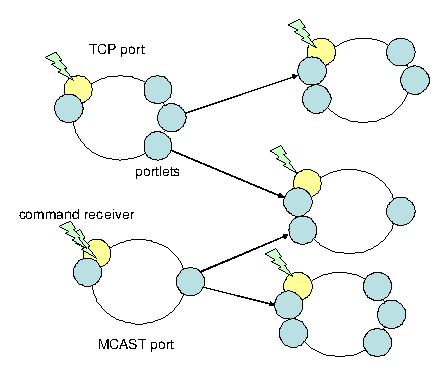
\includegraphics[width=10cm]{fig-port-portlets}
}
\caption[Interprocess communication model]{ 
%
Communications model.  Every process or thread can own
any number of ports.  Every port can be directed to send
data to any number of other ports.  Since different
processes will access this data at different rates,
it is useful to consider each port as owning several
``portlets'' that manage each individual link to another
port.  Given the most conservative quality of service settings,
data will persist in the communications system 
as long as is necessary to send it on the slowest link.
%
}
\label{fig:yarp-port}
\end{figure}

The main abstraction for inter-process communication is called a
port. A port template class can be specialized to send any data type
across an IP-network relying on a set of different
protocols. Depending on the protocol different behaviors can be
obtained the implemented protocols include TCP, UDP, MCAST, QNET1, and
shared memory. A port can either send to many target ports or receive
simultaneously from many other ports. A port is an active object: a
thread continuously services the port object. Being an active object
allows responding to external events at run time, and for example it
is possible to send commands to port objects to change their
behavior. Commands include connecting to another remote port or
receiving an incoming request for connection and since all this can be
done at run-time it naturally enables connecting/disconnecting parts
of the control system on the fly.


Figure~\ref{fig:yarp-port} shows an exemple structure of the port
abstraction. Each port is, in practice, a complex object managing many
communication channels of the same data type. Each port is potentially
both an input and output device although for simplicity of use only
one modality is actually allowed in practice. This is enforced by the
class definition and the C++ type check. Each communication channel is
managed by a portlet object within the main port. Different situations
are illustrated in Figure~\ref{fig:yarp-port}: for example an MCAST
port relies on the protocol itself to send to multiple targets while
on the contrary a TCP port has to instantiate multiple portlets to
connect to multiple targets. In cases where the code detects that two
ports are running on the same machine the IP protocol is replaced by a
shared memory connection. In Figure~\ref{fig:yarp-port} a special
portlet is shown: this is indicated as command receiver. As already
mentioned its function is that of receiving commands to connect,
disconnect, or generically operating on the port. Further ports can
run independently without blocking the calling process (if desired) or
they can wake up the calling process on the occurrence of new data. In
some cases synchronous communication is allowed (TCP protocol).

Protocols can be intermixed following certain rules. Different
operating systems can of course communicate to each other. QNET
protocol is an exception and it is only valid within a QNX network.

YARP communication code leads to a componentization of the control
architecture into many cooperating modules. The data sent through port
can range from simple integral types to complex objects such as arrays
of data (images) or vectors. Thus controlling a robot becomes
something like writing a distributed network of such modules.

In addition, YARP contains supporting libraries for mathematics and
robot type computation (kinematics, matrices, vectors, etc.), image
processing (compatible with the Intel IPL library), and general
purpose utility classes. We also designed a few modules based on
existing Microsoft technology to allow remote controlling Windows
machines (this support comes naturally on QNX). In short, these
scriptable modules complete seamlessly the architecture allowing the
design of scripts to bring up the whole control structure and connect
many modules together.

A Matlab interface to ports has been implemented. This allows building
Matlab modules (e.g. .m files) that connect to the robot to read/write
data. There are basically two advantages: i) complex algorithms can be
quickly implemented and tested relying on Matlab existing toolboxes,
ii) an additional level of scripting can be realized within
Matlab. Matlab provides a relatively efficient and easy to use display
library that can be used to visualize the functioning and performance
of an ongoing experiment.

\subsection{Robot independent code}

One of the goals in writing our control architecture has been that of
simplifying the programming of a complex robotic structure such as a
humanoid robot. Control cards come in many different flavors and
programming them is usually painful. It would be much better if a
standardized interface were provided. It would be even better if a
suitable abstraction were available.

To solve the first problem we defined a virtual device driver
interface into YARP. To solve the second, we encapsulated the control
of parts of the robot (head, arm, frame grabbers, etc.) into a
standardized template class hierarchy.

In short, the virtual device drivers bear much of their structure from
the UNIX device drivers. Each cards driver class contains three main
methods: Open, Close, and IOCtl. The latter is the core of the
interface. Each device accepts a set of messages (with parameters)
through the IOCtl call. Each message accomplishes a specific
function. Two different control cards supporting roughly the same
commands can be easily (as it was done in our setup) mapped into
exactly the same virtual device driver structure, although clearly the
implementation might differ.

The next layer is a C++ hierarchy of classes which through templates
includes both the specification of the controlling device driver
(e.g. the head is controlled through a certain control card) and the
idiosyncrasies of the particular setup (e.g. wiring of the robot might
differ, or initialization might require different calibration
procedures). 


\subsection{Robot specific interface}

The real communication with the robot is carried out through a set of
binary modules that use a device driver structure. Module
customization is at this stage accomplished through configuration
files. In the YARP language these modules are called daemons (a term
borrowed from UNIX). The daemons directly interact with the remainder
of the robot software through YARP ports and in general they export
very specialized communication channels. For example the frame grabber
has an output port of type image and the head control daemon an input
port that accepts velocity commands. There are no specific
restrictions on the type of ports exported by a daemon since any type
of state information about the modules might be required.

Further, some of the daemons accept or send commands of a special type
that are generally used to communicate status information. A bus
structure based on the MCAST protocol has been implemented to transmit
and receive these special messages (called bottles). YARP bottles may
contain any type of data or even a group of heterogeneous elements of
different types. The structure contains identifiers to properly decode
messages and interpret the data. YARP bottles create a network within
the network of behaviors to realize a high-level control and
coordinate a large number of modules.





%%\input{section-from-thesis}

\end{document}

